\documentclass[a4paper, 12pt]{report}

\usepackage[english, greek]{babel}
\usepackage[LGR]{fontenc}
\usepackage{hyphenat}
\usepackage{indentfirst}
\usepackage{geometry}
\usepackage{listings}
\usepackage{xcolor}
\usepackage{amsmath}
\usepackage{graphicx}

\makeatletter
\setlength{\@fptop}{0pt}
\makeatother

\newcommand{\en}{\selectlanguage{english}}
\newcommand{\gr}{\selectlanguage{greek}}

\definecolor{codegreen}{rgb}{0,0.6,0}
\definecolor{codegray}{rgb}{0.5,0.5,0.5}
\definecolor{codepurple}{rgb}{0.58,0,0.82}
\definecolor{backcolour}{rgb}{0.95,0.95,0.92}


% Hyphenation
\hyphenpenalty 10000
\exhyphenpenalty 10000

% Layout
\geometry{a4paper, right = 25mm, left=25mm, top=30mm, bottom = 20mm}

% Cover page
\title{\Large{\textbf{Γραφικά Εργασία 1η}}}
\author{Κόρο Έρικα, 9707}
\date{Απρίλιος 8, 2022}

\begin{document}
    \maketitle

    \section*{Εισαγωγή}
    Σκοπός της εργασίας είναι η υλοποίηση ενός προγράμματος πλήρωσης τριγώνων 
    που σχηματίζουν την προβολή ενός τρισδιάστατου αντικειμένου σε δύο διαστάσεις.
    Η σειρά με την οποία πρέπει να χρωματιστούν τα τρίγωνα προκύπτει από τον πίνακα
    βάθους που δίνεται στο \en numpy \gr αρχείο. Ο χρωματισμός θα ξεκινάει από τα μακρινότερα
    τρίγωνα και θα συνεχίζει με τα κοντινότερα. 
    

    \section*{Σχετικά με τον κώδικα}
    Για την υλοποίηση του προγράμματος χρησιμοποιήθηκε ο \en package manager pip \gr
    και οι βιβλιοθήκες \en numpy \gr και \en matplotlib\gr. Για να τρέξει επιτυχώς ο κώδικας χρειάζεται μέσα στο ίδιο \en
    directory \gr με το \en project \gr να βρίσκεται και το αρχείο \en hw1.npy \gr που μας δίνεται. Το αρχείο αυτό περιέχει τα απαραίτητα δεδομένα 
    για τις κορυφές των τριγώνων, το βάθος των κορυφών και τα χρώματα των κορυφών.
    Μέσα στα αρχεία \en demo\_gouraud.py \gr και
    \en demo\_flat.py \gr δίνεται ο κώδικας για την φόρτωση των δεδομένων. 
    Το \en render \gr της εικόνας παίρνει κάποια δευτερόλεπτα και όταν τελειώσει η εκτέλεση του προγράμματος η είκόνα αποθηκεύεται στο αντίστοιχο αρχέιο.
    


    \section*{Δομή του κώδικα}
    Αρχικά, υλοποιείται η συνάρτηση
    \en interpolate color
    \gr για να υπολογίζει τις χρωματικές συνιστώσες
    ενός σημείου που βρίσκεται ανάμεσα σε δύο σημεία με γνωστές οριζόντιες ή κάθετες συντεταγμένες
    και γνωστές χρωματικές συνιστώσες. Ο τύπος που εφαρμόζεται είναι ο ακόλουθος:
        \begin{align}
          m &= \frac{x\textsubscript{2} - x}{x\textsubscript{2} - x\textsubscript{1}}\\
        value &= m * C\textsubscript{1} + (1 - m) * C\textsubscript{2} 
        \end{align}
        όπου $C\textsubscript{1}$ είναι ο \en R, G, B \gr πίνακας του πρώτου 
    σημείου και $C\textsubscript{2}$ είναι ο \en R, G, B \gr πίνακας του δεύτερου σημείου.
    
    Έπειτα, στο πλαίσιο πραγμάτωσης της συνάρτησης \en shade triangle \gr, υλοποιήθηκε η συνάρτηση
    χάραξης ευθειών \en bresenham, \gr όπως αυτή παρουσιάζεται στις σημειώσεις, με κάποιες τροποποιήσεις
    ώστε να συμπεριληφθεί και η περίπτωση όπου η κλίση της ευθείας είναι μεγαλύτερη της μονάδας.
    Η συνάρτηση αυτή καλείται τρεις φορές μέσα στην \en shade triangle \gr με ορίσματα τις κορυφές του τριγώνου
    για να σχηματιστεί το αντίστοιχο τρίγωνο. Ανάλογα με τον επιθυμητό τρόπο σκίασης \en "flat" \gr ή \en
    "gouraud" \gr που δίνεται σαν είσοδος στην συνάρτηση, χρωματίζονται πρώτα τα \en pixels \gr που βρίσκονται πάνω στις πλευρές
    του τριγώνου με βάση το χρώμα των κορυφών είτε καλώντας την \en interpolate color(gouraud) \gr είτε χρωματίζοντας με το 
    μέσο όρο χρώματος των κορυφών. Στη συνέχεια, ξεκινάει ένας βρόχος επανάληψης για την
    \en scanline \gr η οποία ξεκινάει απ' το μικρότερο \en row \gr των πλευρών του τριγώνου 
    και καταλήγει στο μεγαλύτερο. Μέσα σ' αυτό τον βρόχο, θεωρούμε όλες τις πλευρές
    του τριγώνου ενεργές και σε κάθε επανάληψη βρίσκονται τα ενεργά σημεία της κάθε πλευράς.
    Τέλος, ανάμεσα στα ενεργά σημεία των πλευρών με το μικρότερο \en column \gr χρωματίζονται
    καταλλήλως τα σημεία που βρίσκονται ανάμεσά τους.
    
    Τελευταία υλοποιείται η συνάρτηση \en render \gr. Μέσα σ' αυτή ταξινομείται
    ο πίνακας \en faces \gr, ο οποίος ύστερα από τροποποίηση έχει πλέον τις συντεταγμένες των
    κορυφών κάθε τριγώνου, με βάση το βάθος κάθε τριγώνου για να ξεκινήσει ο χρωματισμός
    των τριγώνων απ' τα μακρινότερα στα κοντινότερα. Αφού έχουν υλοποιηθεί όλα αυτά,
    καλείται η \en shade triangle \gr για τον χρωματισμό όλων των τριγώνων και τον τελικό χρωματισμό του αντικειμένου.

    \lstdefinestyle{mystyle}{
        backgroundcolor=\color{backcolour},   
        commentstyle=\color{codegreen},
        keywordstyle=\color{magenta},
        numberstyle=\tiny\color{codegray},
        stringstyle=\color{codepurple},
        basicstyle=\ttfamily\footnotesize,
        breakatwhitespace=false,         
        breaklines=true,                 
        captionpos=b,                    
        keepspaces=true,                 
        numbers=left,                    
        numbersep=5pt,                  
        showspaces=false,                
        showstringspaces=false,
        showtabs=false,                  
        tabsize=2
    }
    \en
    \lstset{style=mystyle}


\begin{lstlisting} [language = Python]
def shade_triangle(img: list, verts2d: list, vcolors: list,
                        shade_t: str):

    # Call the bresenham algorithm 3 times to shape the triangle
    side1 = bresenham(verts2d[0], verts2d[1])
    side2 = bresenham(verts2d[1], verts2d[2])
    side3 = bresenham(verts2d[2], verts2d[0]) 

    # Shade edges
    if shade_t == "flat":
        # Color each point on the triangle's sides
        for pixel in side1:
            img[pixel[1]][pixel[0]] = list(average_color)
        for pixel in side2:
            img[pixel[1]][pixel[0]] = list(average_color)
        for pixel in side3:
            img[pixel[1]][pixel[0]] = list(average_color)
    elif shade_t == "gouraud":
        # Color the pixels in the edges
        for pixel in sides:
            # If the pixel is not a vertex, use interpolate_color
            if pixel not in verts2d:
                image[pixel] = interpolate_color()
            # else the color of the pixel is in the vcolors list
            else:
                image[pixel] = vcolors
    
    # Find the active points(the colored)
    for scan in range(scan_start, scan_end + 1):
        # Find the edge points that cross with the scanline
            # Hold those points in active_points list
            for i in range(min_col_active + 1, max_col_active):
                # shade the points between min_col_active
                # and max_active_col
                if shade_t == "flat":
                    img[i][scan] = average_color
                    elif shade_t == "gouraud":
                        img[i][scan] =
                            interpolate_color(min_col_active,
                                                max_col_active, i,
                                            img[min_col_active][scan],
                                            img[max_col_active][scan])
            
    
\end{lstlisting}  



\gr Έχοντας ολοκληρώσει τον αλγόριθμο για την πλήρωση τριγώνου, υλοποιείται η συνάρτηση
για τον χρωματισμό του αντικειμένου. Μέσα στον πίνακα \en faces \gr, ύστερα από τροποποιήσεις
βρίσκονται πλέον οι συντεταγμένες των κορυφών κάθε τριγώνου και στον πίνακα \en
depths Of Triangles \gr αποθηκεύονται τα βάθη κάθε τριγώνου. Έπειτα, ταξινομείται ο πίνακας με τα 
βάθη και αντιστοίχως ταξινομείται και ο πίνακας \en faces \gr για να ξεκινήσει ο χρωματισμός.
\newpage

\en
\begin{lstlisting}[language = Python]
def render(verts2d: list, faces: list, vcolors: list, depth: list,
             shade_t: str):
    # Initialize the image
    # Make appropriate changes for faces list
    # Calculate the depth of triangles

    for triangle in faces:
        shade_triangle(image, triangle,
                         triangle_colors[faces.index(triangle)], shade_t)

    \end{lstlisting}

\gr
\section*{Παραδοχές και Παρατηρήσεις}
Λόγω της δομής του αλγορίθμου για την πλήρωση τριγώνου κατά τον οποίο όλες οι πλευρές θεωρούνται ενεργές και λόγω της
παραδοχής ότι κάποια \en pixels \gr που ανήκουν σε περισσότερα από ένα τρίγωνα χρωματίζονται περισσότερες
από μια φορές παίρνει αρκετά δευτερόλεπτα για το \en render \gr της εικόνας. Είναι αρκετά δύσκολο ωστόσο να γνωρίζουμε
εκ των προτέρων ποια \en pixels \gr ανήκουν σε ποια τρίγωνα και να χρωματιστούν μόνο μια φορά. Επίσης, το \en render \gr της εικόνας 
καθυστερεί και λόγω της διαχείρισης κάποιων δεδομένων και της ταξινόμησής τους.



\begin{figure} [!htpb]
    \centering
    
\includegraphics[scale = 0.9]{../pyCharm/flat.png}
    \en
    \caption{flat shading}
\end{figure}

\begin{figure}
    \centering
    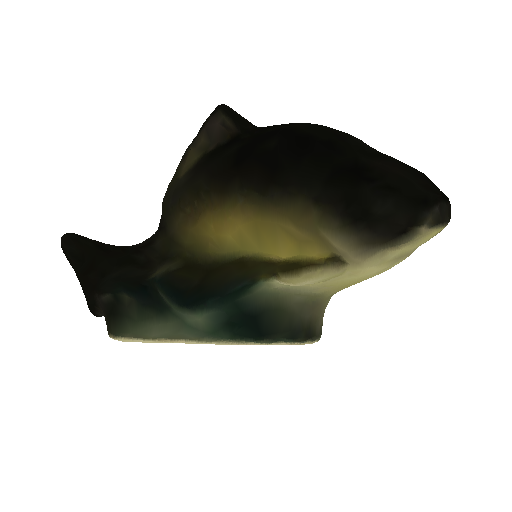
\includegraphics[scale = 0.9]{../pyCharm/gouraud.png}
    \en
    \caption{gouraud shading}
\end{figure}

\end{document}
